\section{Bayesian Neural Networks}\label{BNN}
Neural networks have become increasingly popular in the recent years, due to their ability to
approximate any function arbitrary well (universial approximation theorem). And with the amount of
data in the world today, neural
networks are very powerful regression models for finding the complex patterns. Bayesian neural
network are essentially neural networks, but instead of point estimates, each weight is assigned a
distribution (usually a standard normal distribution), which provides a regression model, 
prior to any observed data. Choosing the prior of a standard normal distribution of a 
3 layers with 10 nodes on each layer the we get the following regression model, 
\begin{figure}
    %\subfloat[\centering prior]{{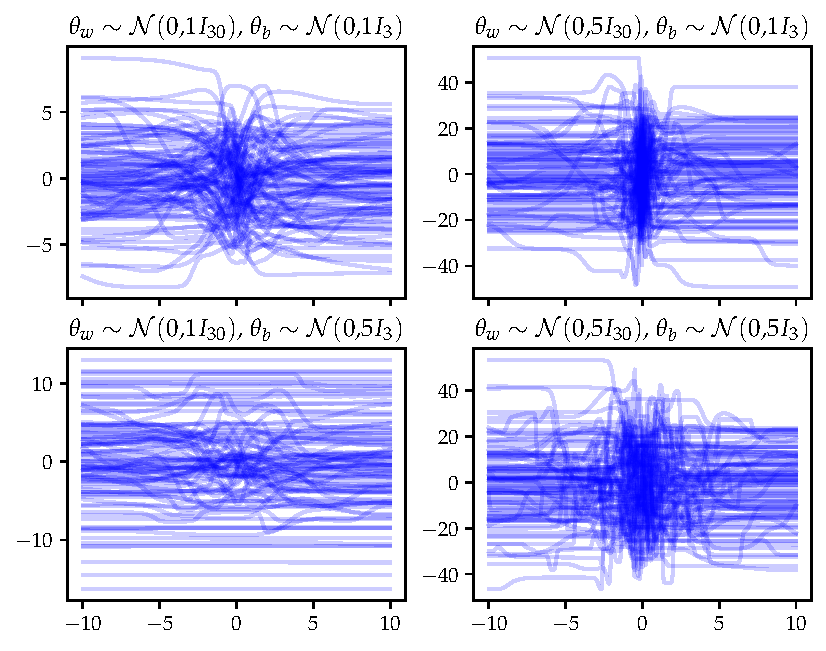
\includegraphics[width=0.45\textwidth]{Pictures/bayesian_nn_prior_samples.pdf} }}%
    %\qquad
    %\subfloat[\centering posterior]{{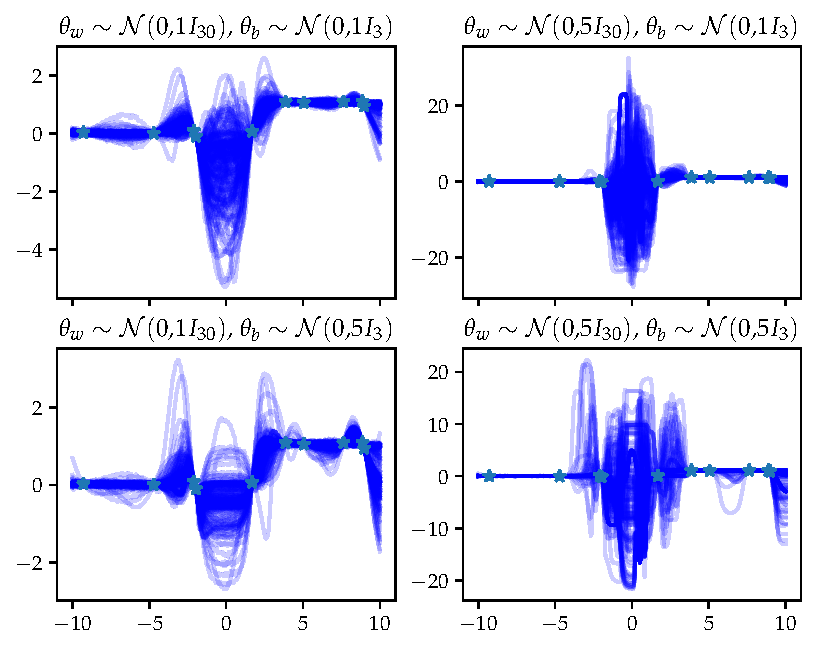
\includegraphics[width=0.45\textwidth]{Pictures/bayesian_nn_posterior_samples.pdf} }}%
    \caption{BNN with $\tan^{-1}(\cdot)$ activation functions and different prior distributions. }%
    \label{fig:example2}%
\end{figure}

\begin{figure}
    \centering
    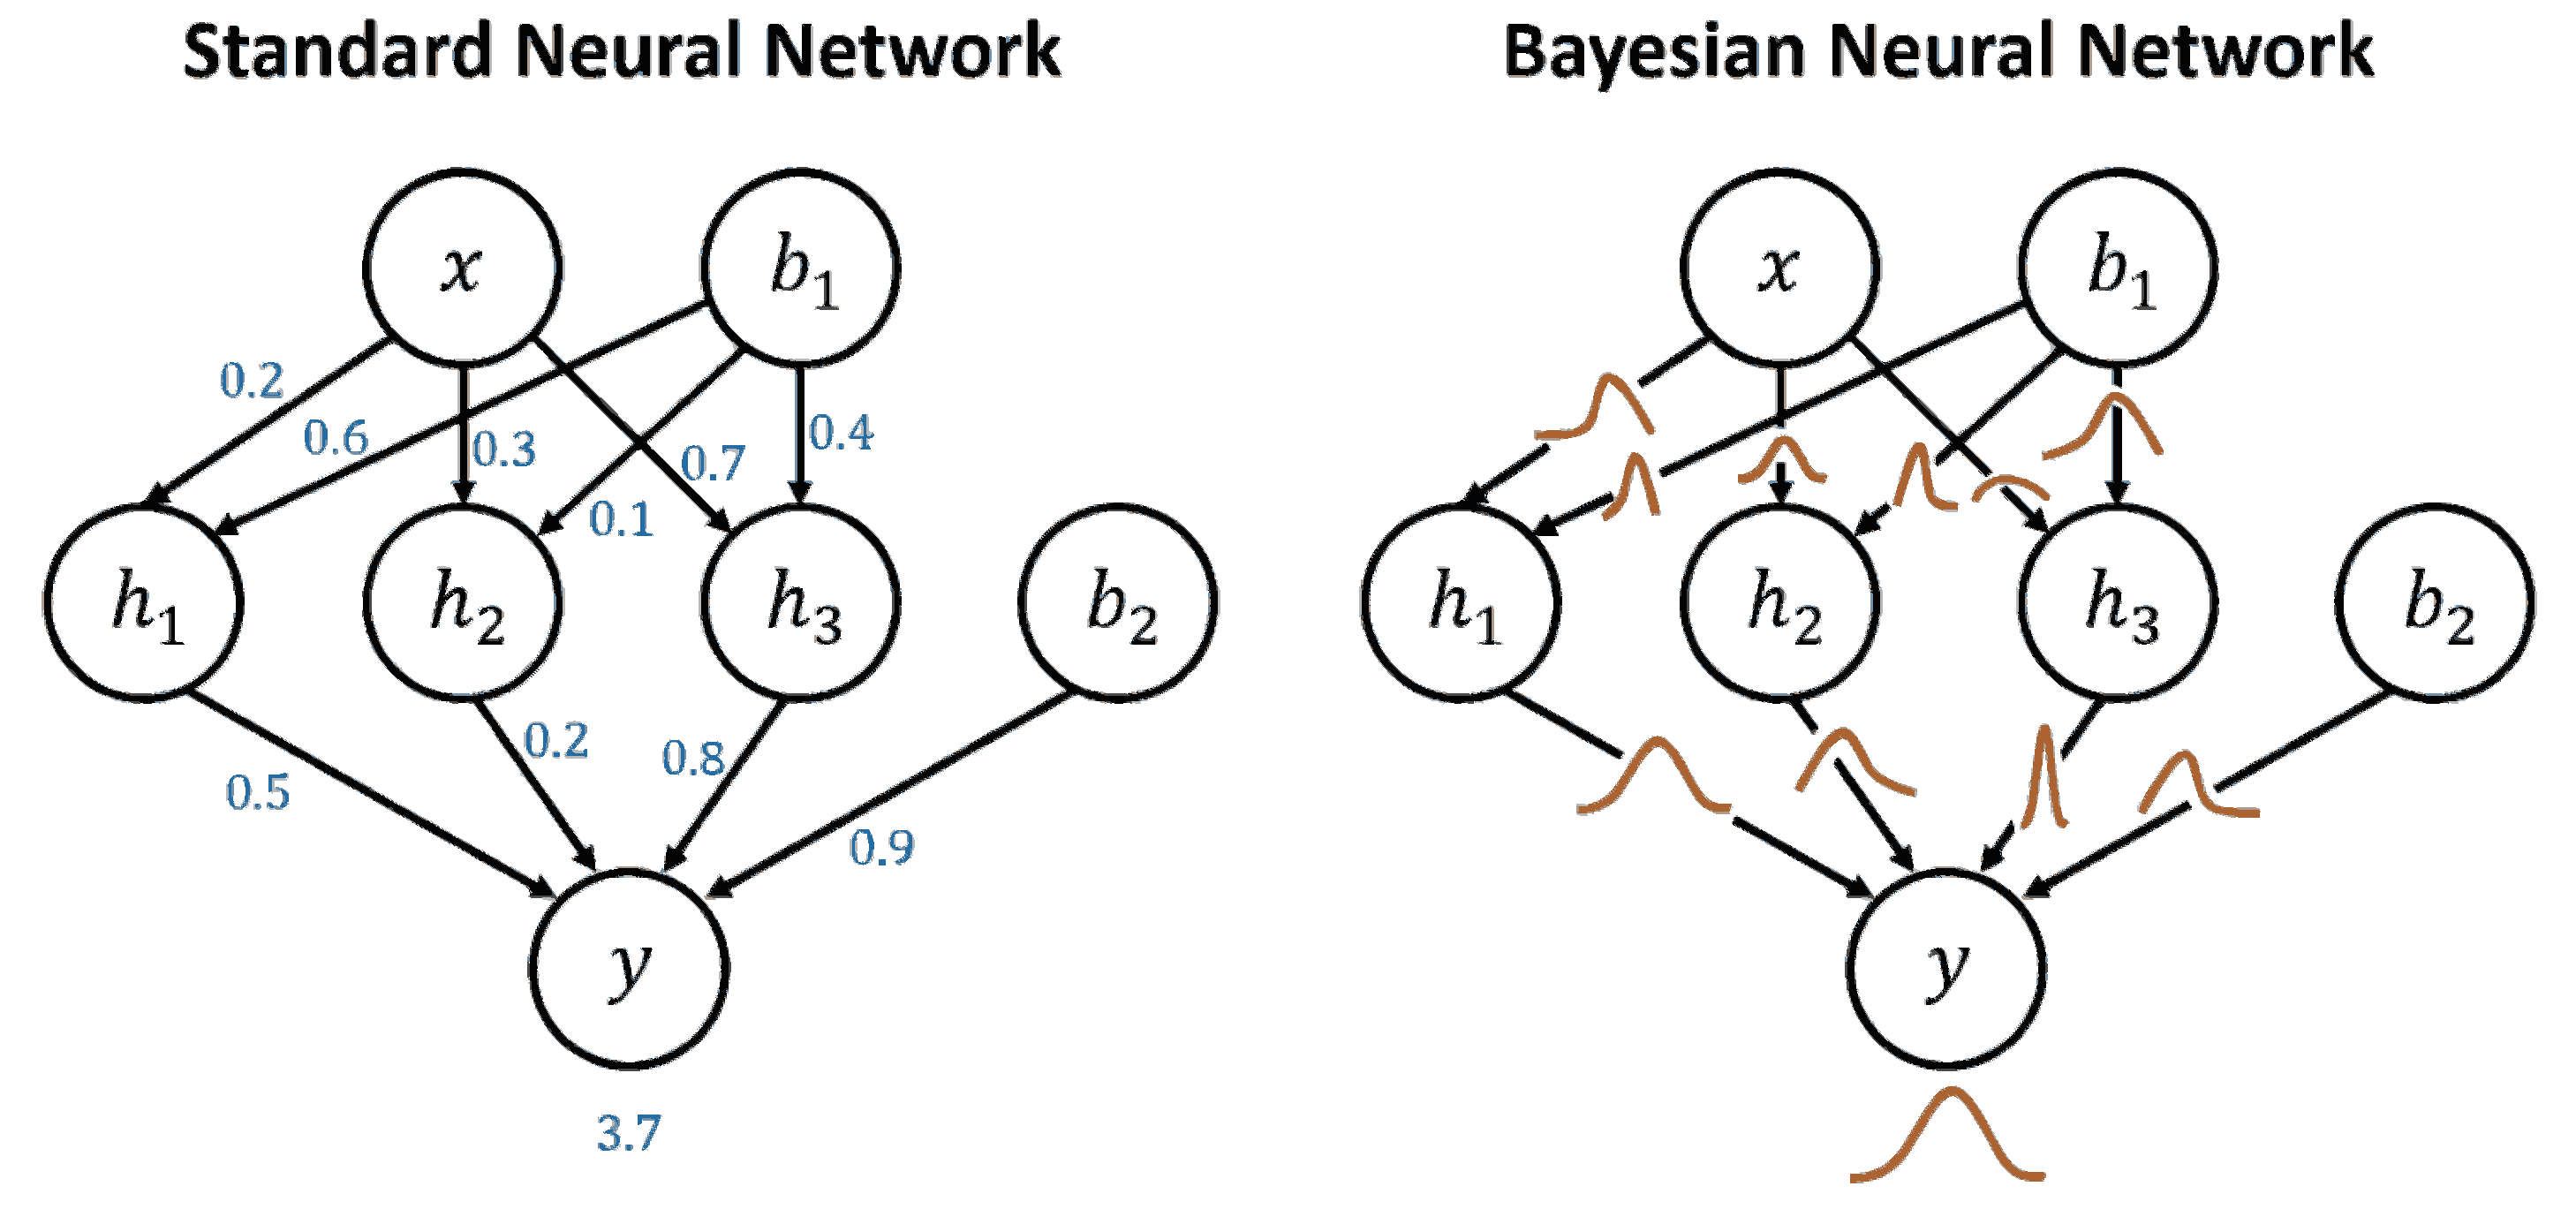
\includegraphics[width=\textwidth]{Pictures/BNN_illustration.pdf}
    \caption*{Bayesian neural network compared to a neural network, were the weights are assigned a
    probability density , note that we often prior assume no correlation and a standard normal
    distribution, but the posterior (after observing data) might contain correlations between the
    weights (i.e. a realization of $w_1$ might influence the realization of $w_2$) (from CYDA)}
\end{figure}

when observing data the distribution of the weights is adjusted accordingly - note that 
there can be correlations between the weights (corresponding to dimension in the distribution). 
The likelihood of a Bayesian Neural network is typically defined as a normal distribution
with mean equal the neural network output (which itself also is a random variabel) and a 
variance random variable $\sigma$ which prior is assumed independent from the input and
assigned a half-caucy or log-normal distribution, 
$$p(y|x, \theta) = \mathcal{N}(y|NN_{w}(x),\sigma^2)$$
Note that the posterior distribution of the weights and $\sigma$ might not be a normal distribution
or anything of the known analytically distributions, it might be highly complex and correlated. 
Therefor BNNs are examples of probabilistic models with intractable inference. The predictive density is given as, 
\begin{align*}
    p(y_*|x_*,\mathcal{D}) &= \int p(y_*|x, \theta)p(\theta|\mathcal{D})d\theta\\
    &\approx \frac{1}{K} \sum_{k=1}^K p(y_*|x, \theta^{(k)})
\end{align*}
where the integral is intractable as $\theta$ can live in a highly dimensional space. The approximation sign
is true, since we can aproximate the integral with monte carlo sampling: $\theta^{(k)}$ are iid samples from the posterior 
distribution, $\theta^{(k)} \sim p(\theta|\mathcal{D})$. We can get samples from the posterior distriution using MCMC

\begin{testexample2}[Monte Carlo approximation]
    Assuming we have a number of iid samples, $\theta^{(1)}, \dots, \theta^{(K)}$ drawn from the
    distribution $p(x)$, then the following appriximation 
    $$E[f(x)] \approx \frac{1}{K} \sum_{k=1}^K f(x^{(k)}) =: \Theta_{K}(f)$$
    holds accoring to the law of large numbers 
    in fact $$E[f(x)] = \lim_{K \rightarrow \infty} \Theta_{K}(f)$$
    and the central limit theorem, <OBS refere!>
    $$p(\hat \Theta) \approx \mathcal{N}(\hat \Theta |\mu_f, \frac{\sigma_f^2}{K})$$
    which ensures that the variance of the unbiased estimator of the expecation decreases
    with number of samples, $K$. Left is to sample the $iid$ samples from the distribution $p(x)$
\end{testexample2}
\subsection*{Posterior samples}
For both models 
the joint distribution $p(\mathcal{D},\theta)$ is available, but calulating the posterior distribution requires the
marginalized likehood, $p(\mathcal{D}) = \int_{\theta} p(\mathcal{D},\theta)$. This integral is often intractable
since the space of $\theta$ typically is abnomous - so not even nummerical appriximations of the intergral is tractable.
From Bayes rule, we have the equality, 
$$p(\theta|\mathcal{D}) = \frac{p(\mathcal{D},\theta)}{p(\mathcal{D})} \propto
p(\mathcal{D},\theta),$$ where the propotional sign is true, since $p(\theta|\mathcal{D})$ is a
function of $\theta$. Knowing the $p(\mathcal{D},\theta)$ joint distribution allow for using Markov
chain Monte Carlo (MCMC) to obtain samples from the posterior distribution.  

\begin{testexample2}[Markov chain Monte Carlo]
    We can conviniently use MCMC for sampling from a probability density $p(x)$, with only the knowledge of a 
    propotional/unnormalised density $\hat p(x) \geq 0$ i.e
    $$\hat p(x) = c\cdot p(x) \hspace{1cm} c = \int \hat p(x) dx,$$
    where $\int \hat p(x) dx$ is a possible intractable integral. 
    An ergodic Markov chain/process is constructed, such that its stationary distribution is exactly $p(x)$, but only
    with the knowledge of $\hat p(x)$. 
\end{testexample2}

\begin{testexample}[Metropolis-Hasting (MH)]
    The most simple MCMC method is the Metropolis-Hasting algorithm. At iteration
    $n$ we have a sample $x_n$,
    \begin{enumerate}
        \item Propose $\hat x$ from a proposal density $q(x_n,\cdot)$
        \item Compute accptance probability $$\alpha(x_n,\hat x) = \min \left(1, \frac{p(\hat x)}{p(x_n)} \frac{q(\hat x, x_n)}{q(x_n,\hat x)}\right)$$
        \item Set the next sample $$x_{n+1} = \begin{cases}
            \hat x &\text{with probability } \alpha(x_n, \hat x)\\
             x_n &\text{with probability } 1-\alpha(x_n, \hat x)
        \end{cases}$$
    \end{enumerate}
    note that $\alpha(x_n,\hat x)$ requires $p(x)$, but since the algorithm only
    requires the fraction $\frac{p(\hat x)}{p(x_n)} = \frac{p(\hat x)\cdot c}{p(x_n)\cdot c} = \frac{\hat p(\hat x)}{\hat p(x_n)}$
    we only need $\hat p$. 
    
    \textbf{Proof:} Assuming discrete states, the transition probability between the states are given as, 
    $$p(x\rightarrow y) = \begin{cases}
        q(x,y)\alpha(x,y) & \text{if } x\neq y\\
        q(x,x) + \sum_{z\neq x} q(x,z)(1-\alpha(x,z)) & \text{if } x=y
    \end{cases}$$
    Now, let us look at the so-called \textit{detailed balance} relation, i.e. that if we are sampling from the
    stationary density we stay there at the next state. Assume $x\neq y$, 
    \begin{align*}
        p(x)p(x\rightarrow y) &= p(x)q(x,y)\alpha(x,y)\\
        &=p(x)q(x,y) \min \left(1, \frac{p(\hat x)}{p(x_n)} \frac{q(\hat x, x_n)}{q(x_n,\hat x)}\right)\\
        &= \min(p(x)q(x,y), p(y)q(y,x))
    \end{align*}
    Observing that the right hand side yields symmetric result in $x$ and $y$, therefore we obtain, 
    $$p(x)p(x\rightarrow y) = p(y)p(y\rightarrow x)$$
    and summing over $x$ on both sides yields,
    \begin{align}
        \sum_x p(x)p(x\rightarrow y) &= p(y) \sum_x p(y\rightarrow x)\\
        \implies \hspace{0.5cm} p(y) &= \sum_x p(x)p(x\rightarrow y)
    \end{align}
    similar conclusion will be obtained for $x = y$, all in all this reveals that $p(x)$ is in fact invariant for the chain
     $\{x_1, \dots , x_n\}$ and thereby that MH is a MCMC algorithm. 
\end{testexample}

% Markov assumption -> history doesn't matter
% Monte Carlo -> Random simulation
% best methods, use gradients. 

% Simulared skate board in a state park. Physic simulation. 
% Often the simulation moves back and fouth and end up in the 
% same point - this is called a U-turn. 

% find global curvature from just knowing the local curvature. 
% Simulation is moving more in the area with high prob. mass. 

% Gradients: Automated differentiation. 

% We want to evaluate integrals of the fom $$E[f(x)] = \int f(x)p(x)dx$$ where $x \in \mathbb{R}^n$ is a
% random vector under the distribution $p(x)$. we are interested in problems where the form of $f(x)$ or $p(x)$
% makes the integral intractalbe. 

% \begin{testexample}[Bayesian neural network]
%     Choosing $f := \mathcal{N}(y;NN_w(x), \sigma)$ and looking at $\theta := (w,\sigma)$ as the random quantaty
%     under the posterior distribution $p(\theta|\mathcal{D})$ we indeed have case of a intractalbe expectation
% \end{testexample}



% Transition density kernel (transtion matrix for finite discrete spaces) $p(x^{(k)}|x^{(k-1)})$



% c) the convergence rate is independent on the
% dimensionality, l. The latter property is in contrast to methods based on the deterministic numerical
% integration, which, in general, have a rate of convergence that slows down as the dimensionality
% increases.

HM with random walk transition is very simple and it comes with some serious disadvantages:
slow convergence speed, might stay in the same region for a long time and produces highly correlated sampels. 
We can do better by replacing the random walk with gradient-guided movements and intepretate the probability
landscape as a physical system.


\begin{testexample}[HMC]
The golden standard in MCMC is the Hamilton monte carlo, which exploits arguments from classical mechanics
around the Hamiltonian equations. This method leads to more efficient sampling as the Hamiltonian intepretation allows the system
to take regions with high probability mass into acound - this is optained using gradient
of the probability landscape.  $\frac{-\partial E(x)}{\partial x} $
 
We define PDF
$$p(x) = \frac{1}{Z_E}\exp(-E(x)),$$

where $E(x)$ is interpretted as the systems potential energy. Now, an latent vector $q$ is introduced in order
to represent the momentum of the system, which gives us the kinetic energy of the system. 

$$K(q) = \frac{1}{2}\sum_{i=1}^l q_i^2$$

Giving the Hamilton function and its coresponing distribution

$$H(x,q)= E(x)+K(q)$$

and 
\begin{align}
    p(x,q) &= \frac{1}{Z_H} \exp(-H(x,q))\\
    &= \frac{1}{Z_E} \exp(-E(x))\frac{1}{Z_K} \exp(-K(x))\\
    &= p(x)p(q)
\end{align}

The desired distribution $p(x)$ is found as the marginal of $p(x,q)$

\end{testexample}

since some intuition is now established around Hamiltonian Monte Carlo, 
we look a bit at the two versions used in Numpyro-BNN and Bohamiann, 

\subsection{No U-Turn sampling}

othen the physical simulation in HMC goes forth and back the same path, and we risk getting bad samples.
No U-turn (NUTS) sampling avoid this. 

\subsection{Adaptive stochatic HMC}
BOHAMIANN is using an adaptive stochastic Hamiltonian monte carlo method to train the BNN. 


\subsection{Design of Bayesian neural network}
The architecture of a BNN is a large topic to discuss. There are certain tradeoffs to be taken into
consideration: How expressive should the network be (i.e. how deep and how many nodes per layer) vs
how much time do we have for the sampler to converge to the true posterior distribution? One very
annoying part of MCMC is that it is very hard to know when the samples are actually true samples
from the posterior. A consideration when training deterministic neural networks are overfitting
however this is not a big consideration when fitting Bayesian neural networks; Choosing a prior
around 0 will regulate the parameters, and thereby postpone overfitting. 

This thesis is inspired by the PhD thesis \cite{PhDthesis}, which uses an architecture of a 2 layers
with 50 sigmoid-nodes in each layer, and the BOHAMIANN paper \cite{BOHAMIANN}, default uses an architecture
of 3 layers with 50 tanh-nodes in each layer. As we want to make sure always to do the 
inference correctly, we want to be able to take a proper amount of samples, while also
have an explicit model. Figure \eqref{n_unit_BNN} shows prior samples of BNN with a different
number of tanh-nodes on each of the 3 layers, this provides an intuition that choosing a larger
BNN leads to a more expressive regression model. When doing Bayesian optimization it is very limited
amount of training data, i.e. complicated patterns in data is not possible to discover, and hence 
highly expressive models are not important. 



\begin{figure}[H]
    \centering
    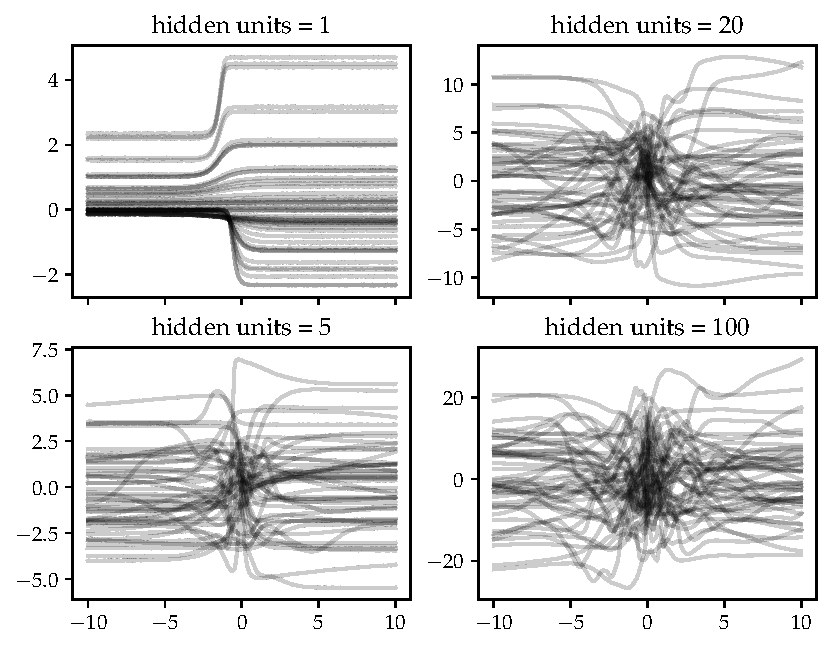
\includegraphics[width=\textwidth]{Pictures/bayesian_nn_prior_samples_hidden_units.pdf}
    \caption{Number of units in each of the 3 layers have a large influence of the BNNs ability to be expressive}
    \label{n_unit_BNN}
\end{figure}

Here is the test function 4, where the sampled using 50 points
\begin{figure}[h]
    \centering
    \begin{minipage}[b]{0.49\textwidth}
     \includegraphics[trim=1cm 0.7cm 1cm 1cm,clip,width=\textwidth]{Figures/reg_illustrations/BayesianNN_plots/Test4_BNN500-500-hu-10-alpha-1000_n_100_seed_42.pdf}
    \end{minipage}
    \hfill
    \begin{minipage}[b]{0.49\textwidth}
      \includegraphics[trim=1cm 0.7cm 1cm 1cm,clip,width=\textwidth]{Figures/reg_illustrations/BayesianNN_plots/Test4_BNN500-500-hu-50-alpha-1000_n_100_seed_42.pdf}
     \end{minipage}
     \caption{Example where 100 nodes on each of three layers, lead to a much more expressive model.
     $\sigma^2$ follows a informative prior $InvGamma(1000,1)$, i.e. prior mean $E[\sigma^2] \approx
     \frac{1}{1000}$, and variance $\approx \frac{1}{1000^3}$, however since the data is distributed in such 
     a complex way the limited expressiveness of the model, forces the model to infer make $\sigma^2$ large, 
     i.e. including the data in the noise}
\end{figure}

Another variance! Sometimes the complexity of the problem is incapsled as noise.


\subsubsection{Number of samples}
The number of MCMC samples is of large importance. Theoretically speaking the more samples the better
however, 


\begin{figure}[h]
    \centering
    \begin{minipage}[b]{0.49\textwidth}
     \includegraphics[trim=1cm 0.7cm 1cm 1cm,clip,width=\textwidth]{Figures/reg_illustrations/BOHAMIANN/Test1_BOHAMIANN_n_10_seed_42.jpg}
    \end{minipage}
    \hfill
    \begin{minipage}[b]{0.49\textwidth}
      \includegraphics[trim=1cm 0.7cm 1cm 1cm,clip,width=\textwidth]{Figures/reg_illustrations/BOHAMIANN/Test2_BOHAMIANN_n_40_seed_42.jpg}
     \end{minipage}
    
     \begin{minipage}[b]{0.49\textwidth}
      \includegraphics[trim=1cm 0.7cm 1cm 1cm,clip,width=\textwidth]{Figures/reg_illustrations/BOHAMIANN/Test3_BOHAMIANN_n_40_seed_42.jpg}
     \end{minipage}
     \hfill
     \begin{minipage}[b]{0.49\textwidth}
       \includegraphics[trim=1cm 0.7cm 1cm 1cm,clip,width=\textwidth]{Figures/reg_illustrations/BOHAMIANN/Test4_BOHAMIANN_n_40_seed_42.jpg}
      \end{minipage}
      \caption{BOHAMIANN tested on all problems.}
\end{figure}


\begin{figure}[h]
    \centering
    \begin{minipage}[b]{0.49\textwidth}
     \includegraphics[trim=1cm 0.7cm 1cm 1cm,clip,width=\textwidth]{Figures/reg_illustrations/numpyroBNN/Test1_numpyro_BNN_n_10_seed_42.jpg}
    \end{minipage}
    \hfill
    \begin{minipage}[b]{0.49\textwidth}
      \includegraphics[trim=1cm 0.7cm 1cm 1cm,clip,width=\textwidth]{Figures/reg_illustrations/numpyroBNN/Test2_numpyro_BNN_n_40_seed_42.jpg}
     \end{minipage}
    
     \begin{minipage}[b]{0.49\textwidth}
      \includegraphics[trim=1cm 0.7cm 1cm 1cm,clip,width=\textwidth]{Figures/reg_illustrations/numpyroBNN/Test3_numpyro_BNN_n_40_seed_42.jpg}
     \end{minipage}
     \hfill
     \begin{minipage}[b]{0.49\textwidth}
       \includegraphics[trim=1cm 0.7cm 1cm 1cm,clip,width=\textwidth]{Figures/reg_illustrations/numpyroBNN/Test4_numpyro_BNN_n_40_seed_42.jpg}
      \end{minipage}
      \caption{numpyro BNN tested on all problems.}
\end{figure}